
%% paper.tex
%% for ISORC 2016
%% 2016/11/29
%% by Takuro Yamamoto

\documentclass[conference]{IEEEtran/IEEEtran}
% Some Computer Society conferences also require the compsoc mode option,
% but others use the standard conference format.
%
% If IEEEtran.cls has not been installed into the LaTeX system files,
% manually specify the path to it like:
% \documentclass[conference]{../sty/IEEEtran}

% Package List
%\usepackage[dvips]{graphics}
\usepackage[dvipdfmx]{graphicx}
\usepackage{amssymb}
\usepackage{float}
\usepackage{enumerate,cite,url}
\usepackage{listings,jlisting}
\lstset{%
    language={c},%
    basicstyle={\small\ttfamily},%
    identifierstyle={\small},%
    commentstyle={\footnotesize\itshape},%
    keywordstyle={\small},%\bfseries},%
    ndkeywordstyle={\small},%
    stringstyle={\small\it},
    frame={tb},
    breaklines=true,
    columns=[l]{fullflexible},%
    numbers=left,%
    xrightmargin=0zw,%
    xleftmargin=3zw,%
    numberstyle={\scriptsize},%
    stepnumber=1,
    numbersep=1zw,%
    lineskip=-0.5ex%
}

% *** Do not adjust lengths that control margins, column widths, etc. ***
% *** Do not use packages that alter fonts (such as pslatex).         ***
% There should be no need to do such things with IEEEtran.cls V1.6 and later.
% (Unless specifically asked to do so by the journal or conference you plan
% to submit to, of course. )


% correct bad hyphenation here
\hyphenation{op-tical net-works semi-conduc-tor}


\begin{document}
%
% paper title
% Titles are generally capitalized except for words such as a, an, and, as,
% at, but, by, for, in, nor, of, on, or, the, to and up, which are usually
% not capitalized unless they are the first or last word of the title.
% Linebreaks \\ can be used within to get better formatting as desired.
% Do not put math or special symbols in the title.
\title{TINET+TECS: Component-based TCP/IP Protocol Stack for Embedded Systems}


% author names and affiliations
% use a multiple column layout for up to three different
% affiliations
\author{\IEEEauthorblockN{Takuro Yamamoto}
\IEEEauthorblockA{Graduate School of Engineering Science,\\Osaka University}
\and
\IEEEauthorblockN{Takuma Hara}
\IEEEauthorblockA{}
\and
\IEEEauthorblockN{Takuya Ishikawa}
\IEEEauthorblockA{}
\and
\IEEEauthorblockN{Hiroshi Oyama}
\IEEEauthorblockA{OKUMA Corporation}
\and
\IEEEauthorblockN{Hiroaki Takada}
\IEEEauthorblockA{}
\and
\IEEEauthorblockN{Takuya Azumi}
\IEEEauthorblockA{Graduate School of Engineering Science,\\Osaka University}
}

% conference papers do not typically use \thanks and this command
% is locked out in conference mode. If really needed, such as for
% the acknowledgment of grants, issue a \IEEEoverridecommandlockouts
% after \documentclass

% for over three affiliations, or if they all won't fit within the width
% of the page, use this alternative format:
% 
% \author{\IEEEauthorblockN{Michael Shell\IEEEauthorrefmark{1},
% Homer Simpson\IEEEauthorrefmark{2},
% James Kirk\IEEEauthorrefmark{3}, 
% Montgomery Scott\IEEEauthorrefmark{3} and
% Eldon Tyrell\IEEEauthorrefmark{4}}
% \IEEEauthorblockA{\IEEEauthorrefmark{1}School of Electrical and Computer Engineering\\
% Georgia Institute of Technology,
% Atlanta, Georgia 30332--0250\\ Email: see http://www.michaelshell.org/contact.html}
% \IEEEauthorblockA{\IEEEauthorrefmark{2}Twentieth Century Fox, Springfield, USA\\
% Email: homer@thesimpsons.com}
% \IEEEauthorblockA{\IEEEauthorrefmark{3}Starfleet Academy, San Francisco, California 96678-2391\\
% Telephone: (800) 555--1212, Fax: (888) 555--1212}
% \IEEEauthorblockA{\IEEEauthorrefmark{4}Tyrell Inc., 123 Replicant Street, Los Angeles, California 90210--4321}}

% use for special paper notices
%\IEEEspecialpapernotice{(Invited Paper)}

% make the title area
\maketitle

% As a general rule, do not put math, special symbols or citations
% in the abstract
\begin{abstract}

Embedded systems are applied to Internet of Things (IoT), and the high productivity of embedded network software is required.

TINET is a TCP/IP protocol stack for embedded systems.
TINET is a compact TCP/IP protocol stack, however consists of many complex source codes.
Therefore, it is difficult to maintain, extend, and analysis the software.

To improve the scalability and configurability, this paper has proposed a component-based TCP/IP protocol stack for embedded systems: TINET componentized with TOPPERS embedded component system (TECS).
The component-based TINET provides software developers high productivity such as change of network buffer size and add/remove TCP (or UDP) function.
We evaluate the component-based TINET compared with the original TINET, and confirm that the overheads of execution time and memory consumption are low and  that the configurability is improved.

In this paper, we also demonstrates a use case of the dynamic component connection method of TECS with a network application.

\end{abstract}

% no keywords

% For peer review papers, you can put extra information on the cover
% page as needed:
% \ifCLASSOPTIONpeerreview
% \begin{center} \bfseries EDICS Category: 3-BBND \end{center}
% \fi
%
% For peerreview papers, this IEEEtran command inserts a page break and
% creates the second title. It will be ignored for other modes.
\IEEEpeerreviewmaketitle

\section{Introduction}
\label{sec:Introduction}

Internet of Things (IoT) is an essential keyword for the next era.
Such as wearable devices, smart devices, and smart homes, various things are connected to the Internet, enriching our lives.
Embedded systems are the elements constituting IoT, e.g., sensing data and controlling actuators.
Therefore, embedded network software is required for the high productivity and quality.

TINET (Tomakomai InterNETworking) is a compact TCP/IP protocol stack for embedded systems \cite{url:TINET}.
TINET supports the ability such as minimum copy frequency and elimination of dynamic memory control.
TINET needs small memory for its TCP/IP protocol stack, therefore it is suitable for embedded systems.
However, there are several issues that TINET consists of many complex source codes.
It may take a lot of time for software developers to maintain, extend, and analysis the software because TINET is composed of many files and defines many macros.

Component-based development is an approach to improve software productivity.
Component-based development is a design technique that can be applied to reusable software development \cite{par:CBD}, such as TECS \cite{par:TECS}, AUTOSAR \cite{url:AUTOSAR}, and SaveCCM \cite{par:SAVEapproach}.
Component-based systems are flexible to software extension and specification changes.
In addition, individual Component diagrams enable the visualization of an entire system.

In this paper, component-based TCP/IP protocol stack, i.e., componentized TINET, is proposed to improve the configurability and scalability of software.
TECS (TOPPERS Embedded Component System) \cite{par:TECS} is utilized to componentize TINET, because TECS is a component system suitable for embedded systems.
TECS supports static configuration, that component behaviors and interconnections are defined statically, thus TECS can optimize the overhead of componentization.


{\bf Contributions:} This paper provides the following contributions.

\begin{enumerate}

    \item {\bf Improve configurability}\mbox{}\\
        TINET+TECS is a component-based system, therefore the software is flexible to change the configuration such as resize network buffer, add/remove TCP (or UDP) functions, and support both IPv4 and IPv6.
        In addition, a component diagram provides visualization of TINET, a complicated system.

    \item {\bf Dynamic connection method}\mbox{}\\
        

    \item {\bf Support legacy codes}\mbox{}\\
        TECS supports the adapter to call TECS functions from C codes, thus TINET+TECS can use an existing application.
    % \item {\bf Software visualization}

\end{enumerate}

{\bf Organization}: The remainder of this paper is organized as follows.
Section \ref{sec:Basic Technology} introduces the basic technologies, i.e., TINET and TECS.
Section \ref{sec:Design and Implementation} describes the design and implementation of the proposed framework.
Section \ref{sec:Evaluation and Demonstration} evaluates the proposed framework.
Related work is discussed in Section \ref{sec:Related Work}.
Conclusions and suggestions for future work are presented in Section \ref{sec:Conclusion}.


\section{Basic Technology}
\label{sec:Basic Technology}

\subsection{TINET}

TINET is a compact TCP/IP protocol stack for embedded systems based on the ITRON TCP/IP API Specification \cite{url:ITRON_TCP/IP_API_Spec}, developed by TOPPERS (Toyohashi OPen Platform for Embedded Real-time Systems) Project \cite{url:TOPPERS}.
To take restrictions for embedded systems such as memory capacity, size, and power consumption, TINET supports following functions:

\begin{enumerate}
    \item Minimum copy frequency
    \item Elimination of dynamic memory control
    \item Asynchronous interface
    \item Error detailed per API
\end{enumerate}


TINET runs as middleware on TOPPERS/ASP3 \cite{url:ASP3}, a realtime kernel.
TINET has been released as open source.

\subsubsection{Overview}

Fig. \ref{fig:TINET_Hier} shows the hierarchy diagram of TINET and TOPPERS/ASP3.

\begin{figure}[t]
    \centering
    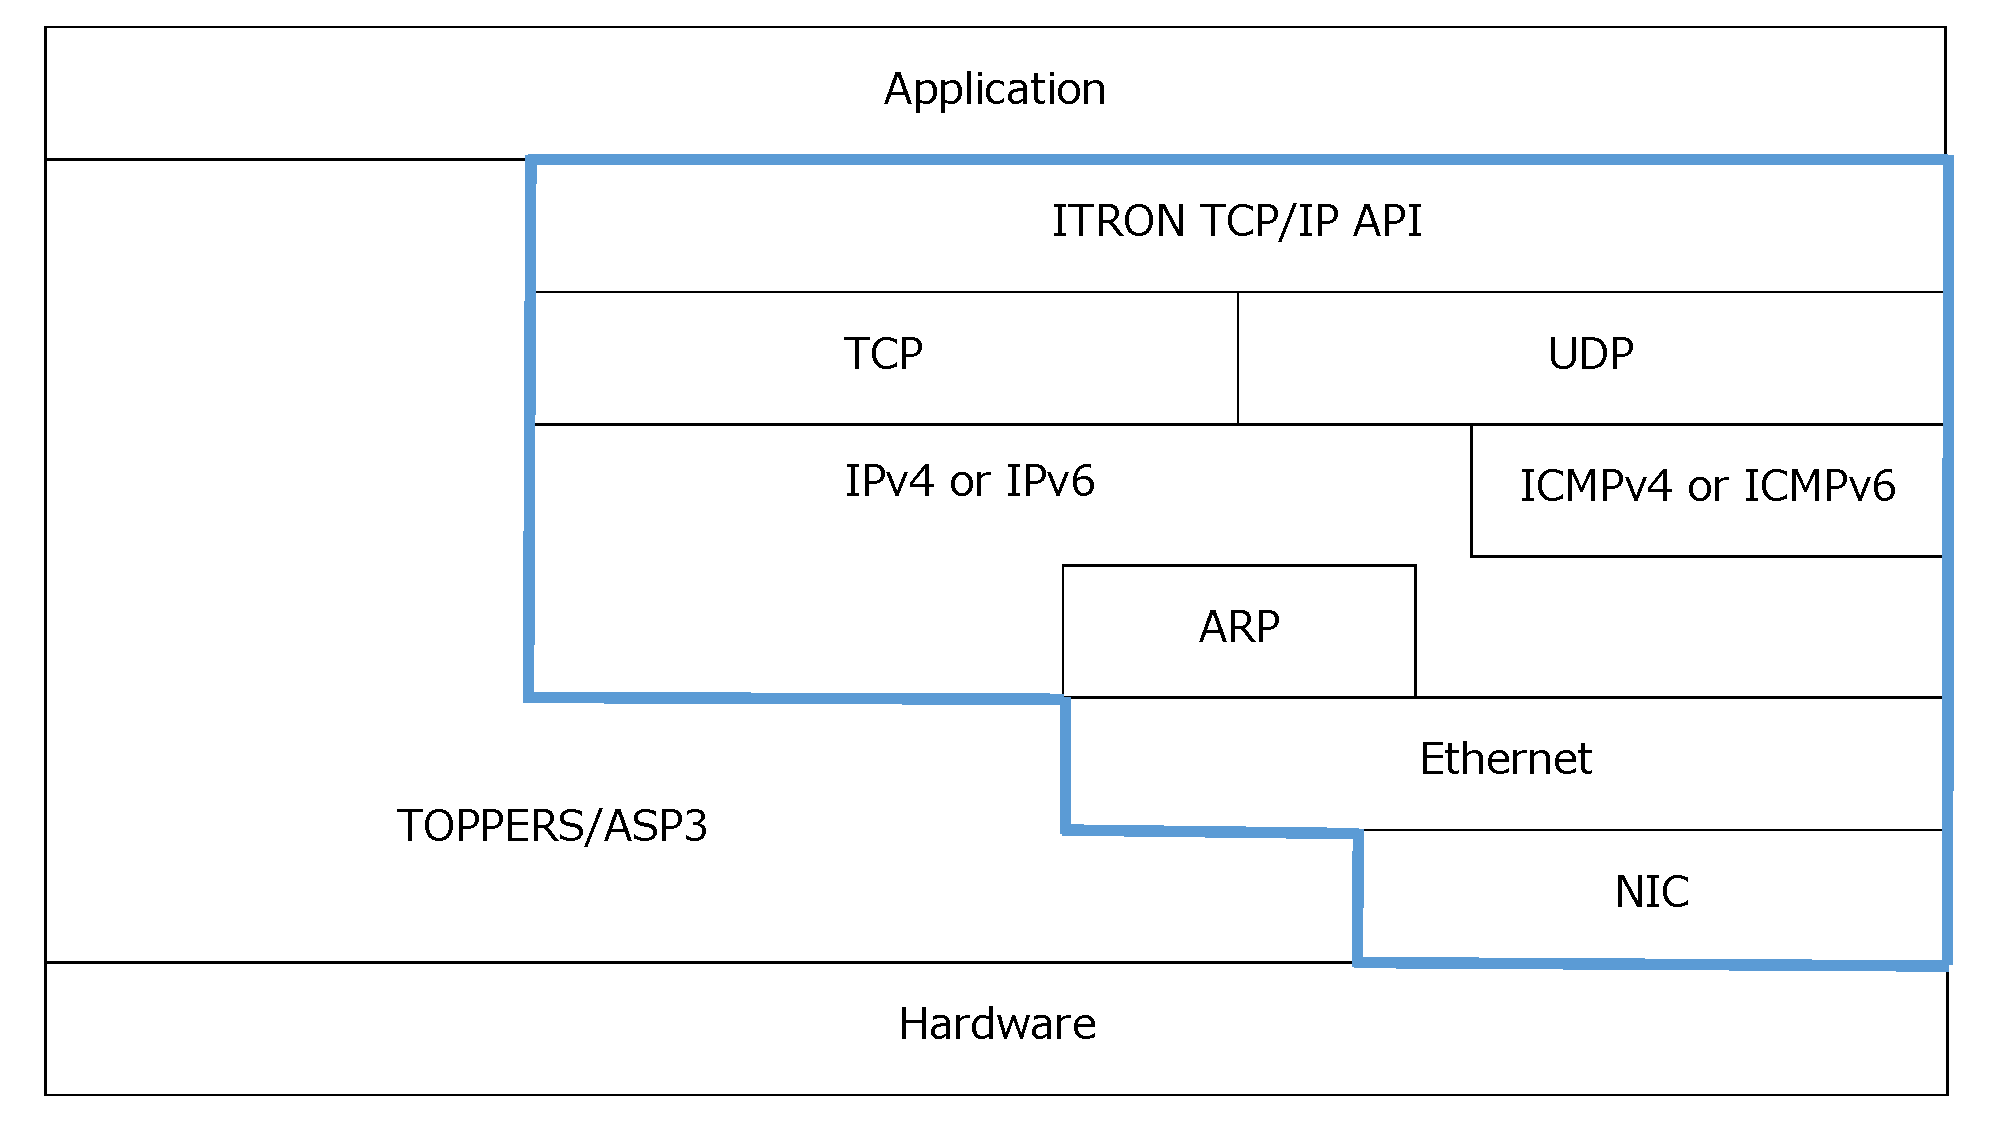
\includegraphics[width=6.5cm,clip]{figure/TINET_Hier.pdf}
    \caption{Hierarchy Diagram of TINET and TOPPERS/ASP3}
    \label{fig:TINET_Hier}
\end{figure}


\subsection{TECS}
\label{sec:TECS}

TECS is a component system suitable for embedded systems.
TECS can increase productivity and reduce development costs due to improved reusability of software components.
TECS also provides component diagrams, which help developers visualize the overall structure of a system.

In TECS, component deployment and composition are performed statically.
Consequently, connecting components does not incur significant overhead and memory requirements can be reduced.
TECS can be implemented in C, and demonstrates various feature such as source level portability and fine-grained components.

\begin{figure}[t]
    \centering
    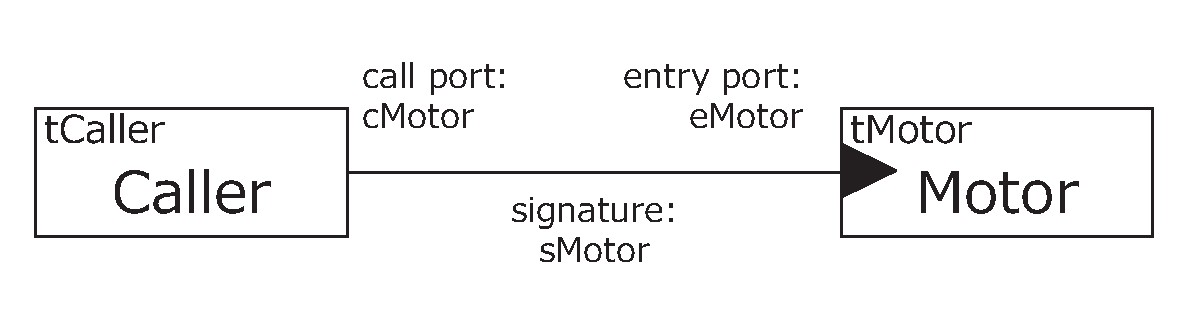
\includegraphics[width=6.5cm,clip]{figure/component_diagram.eps}
    \caption{Component Diagram}
    \label{fig:component}
\end{figure}

\subsubsection{Component Model}

Fig.\ref{fig:component} shows a component diagram.
A {\it cell}, which is an instance of a component in TECS, consists of {\it entry} ports, {\it call} ports, attributes and internal variables.
An {\it entry} port is an interface that provides functions to other {\it cell}s, and a {\it call} port is an interface that enables the use of other {\it cell}'s functions.
A {\it cell} has one or more {\it entry} ports and {\it call} ports.
{\it Cell} functions are implemented in C.

The type of {\it entry}/{\it call} port is defined by a {\it signature}, which is a set of functions.
A {\it signature} is the interface definition of a {\it cell}.
The {\it cell}'s  {\it call} port can be connected to the {\it entry} port of another {\it cell} by the same {\it signature}.
Here, {\it celltype} defines one or more {\it call}/{\it entry} ports, attributes, and internal variables of a {\it cell}.


\subsubsection{Component Description}

In TECS, components are described by {\it signature}, {\it celltype}, and build written in component description language (CDL).
These components are described as follows.

\begin{description}
    \item[{\bf Signature Description}]\mbox{}\\
        The {\it signature} defines a {\it cell} interface.
        The {\it signature} name follows the keyword {\it signature} and takes the prefix ``s'' e.g., sMotor (Fig.\ref{signature}).
        In TECS, to clarify the function of an interface, specifiers such as [in] and [out] are used, which represent input and output, respectively.
\begin{figure}[t]
\centering
\begin{lstlisting}
signature sMotor {
    int32_t getCounts( void );
    ER resetCounts( void );
    ER setPower( [in]int power );
    ER stop( [in] bool_t brake );
    ER rotate( [in] int degrees,
               [in] uint32_t speed_abs,
                [in] bool_t blocking );
    void initializePort( [in]int32_t type );
};
\end{lstlisting}
\caption{Signature Description}
\label{signature}
\end{figure}
    \item[{\bf Celltype Description}]\mbox{}\\
        The {\it celltype} defines {\it entry} ports, {\it call} ports, attributes, and variables.
        A {\it celltype} name with the prefix ``t'' follows the keyword {\it celltype}, e.g., tCaller (Fig.\ref{celltype}).
        To define {\it entry} ports, a {\it signature}, e.g., sMotor, and an {\it entry} port name, e.g., eMotor, follow the keyword {\it entry}.
        {\it Call} ports are defined similarly.
        Attributes and variables follow the keywords {\it attr} and {\it var}, respectively.
\begin{figure}[t]
\centering
\begin{lstlisting}
celltype tCaller {
    call sMotor cMotor;
};
celltype tMotor {
    entry sMotor eMotor;
    attr {
        int32_t port;
    };
    var {
        int32_t currentSpeed = 0;
    };
};
\end{lstlisting}
\caption{Celltype Description}
\label{celltype}
\end{figure}
    \item[{\bf Build Description}]\mbox{}\\
        The build description is used to instantiate and connect {\it cell}s.
        Fig.\ref{build} shows an example of a build description.
        A {\it celltype} name and {\it cell} name, e.g., tMotor and Motor, respectively, follow the keyword {\it cell}.
        To compose {\it cell}s, a {\it call} port, {\it cell}'s name, and an {\it entry} port are described in that order.
        In Fig.\ref{build}, {\it entry} port eMotor in {\it cell} Motor is connected to {\it call} port cMotor in {\it cell} Caller.
        {\it C\_EXP} calls macros defined in C files.

\begin{figure}[t]
\centering
\begin{lstlisting}
cell tMotor Motor {
    port = C_EXP("PORT_A");
};
cell tCaller Caller {
    cMotor = Motor.eMotor;
};
\end{lstlisting}
\caption{Build Description}
\label{build}
\end{figure}

\end{description}

\section{Design and Implementation}
\label{sec:Design and Implementation}

\subsection{send, receive specifier}

TECS supports send and receive specifiers, which are interface specifiers \cite{par:RPC}.
TINET+TECS uses send and receive specifiers instead of in and out to reduce the number of copies.

in is a specifier for input arguments.
A callee side uses the memory of arguments with in while executing the callee function.
When the processing returns to the caller side, the caller can reuse and deallocate the memory.

send is also a specifier for transferring data to a callee from a caller such as in.
The difference between in and send is whether to deallocate the data memory in caller or callee, shown as Figure \ref{fig:SendReceive}.
In case of in specifier, both allocating and deallocating the data memory are performed in the caller.
On the other hand, in case of send, the caller allocates the data memory and the callee deallocates it.

out is a specifier for output arguments.
A callee writes data in the memory allocated by a caller, and the caller receives the data.

receive is also a specifier for a caller receiving data from a callee such as out.
The difference between out and receive is whether to allocate the data memory in caller or callee, shown as Figure \ref{fig:SendReceive}.
While, in case of out, a callee writes data in the memory allocated by a caller, in case of receive, the callee allocates the data memory.
Deallocating the memory is performed in the caller in both cases.

\begin{figure}[t]
    \centering
    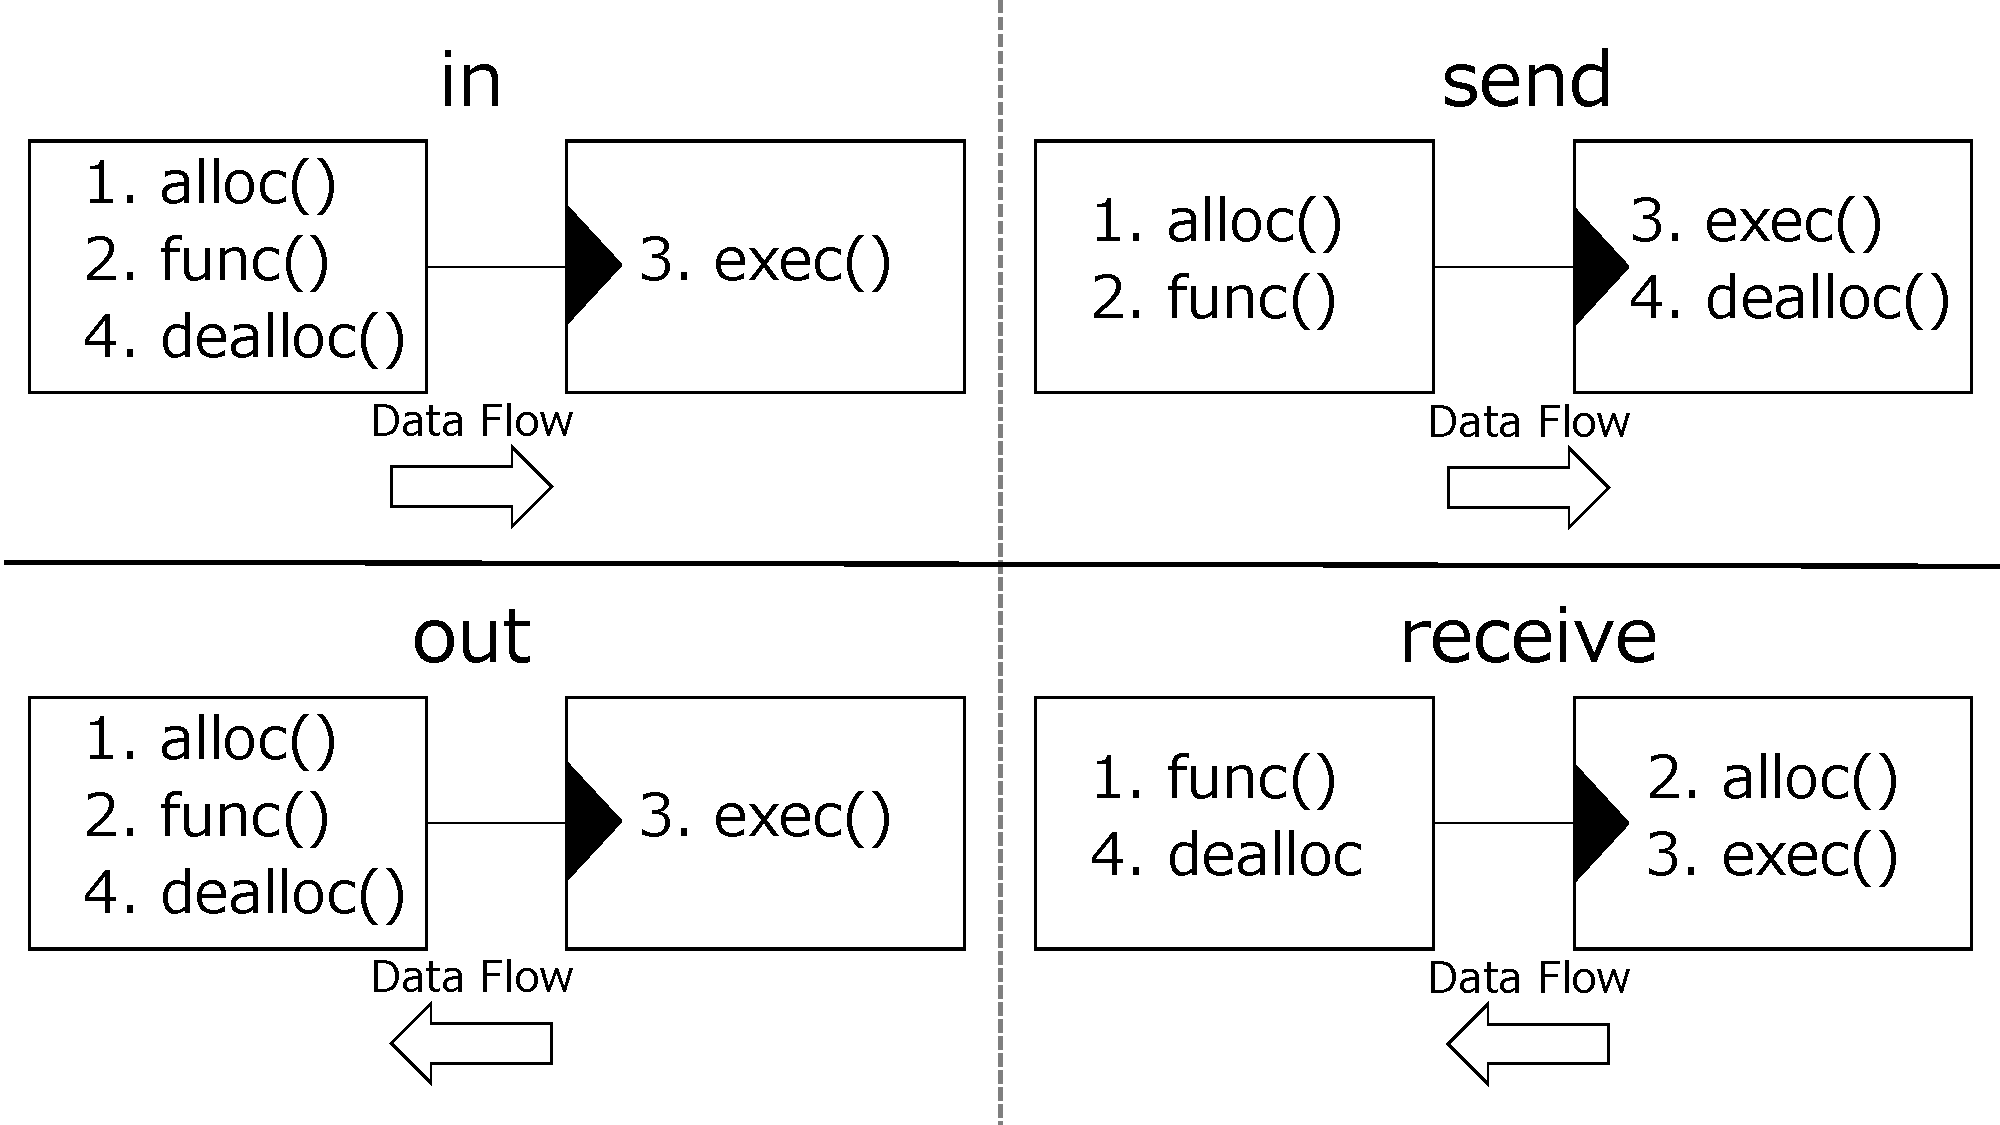
\includegraphics[width=6.5cm,clip]{figure/SendReceive.pdf}
    \caption{Differences between in/out and send/receive}
    \label{fig:SendReceive}
\end{figure}

\begin{figure}[t]
\centering
\begin{lstlisting}
signature sNicDriver {
  void start([send(sNetworkAlloc),size_is(size)]int8_t *outputp,
             [in]int32_t size,
             [in]uint8_t align);
  void read([receive(sNetworkAlloc),size_is(*size)]int8_t **inputp,
            [out]int32_t *size,
            [in]uint8_t align);
    /* Omit: other functions */
};
\end{lstlisting}
\caption{An example of send and receive}
\label{src:SendReceive}
\end{figure}


\subsection{TECS Adapter}

TECS supports {\it Adapter} functionality which enables to call a function in TECS from C codes.
An adapter connects a TECS component, links a C function to a TECS function shown as Fig. \ref{fig:TECS_Adapter}.
Software developers can utilize an existing application for TECS owing to the adapter.

\begin{figure}[t]
    \centering
    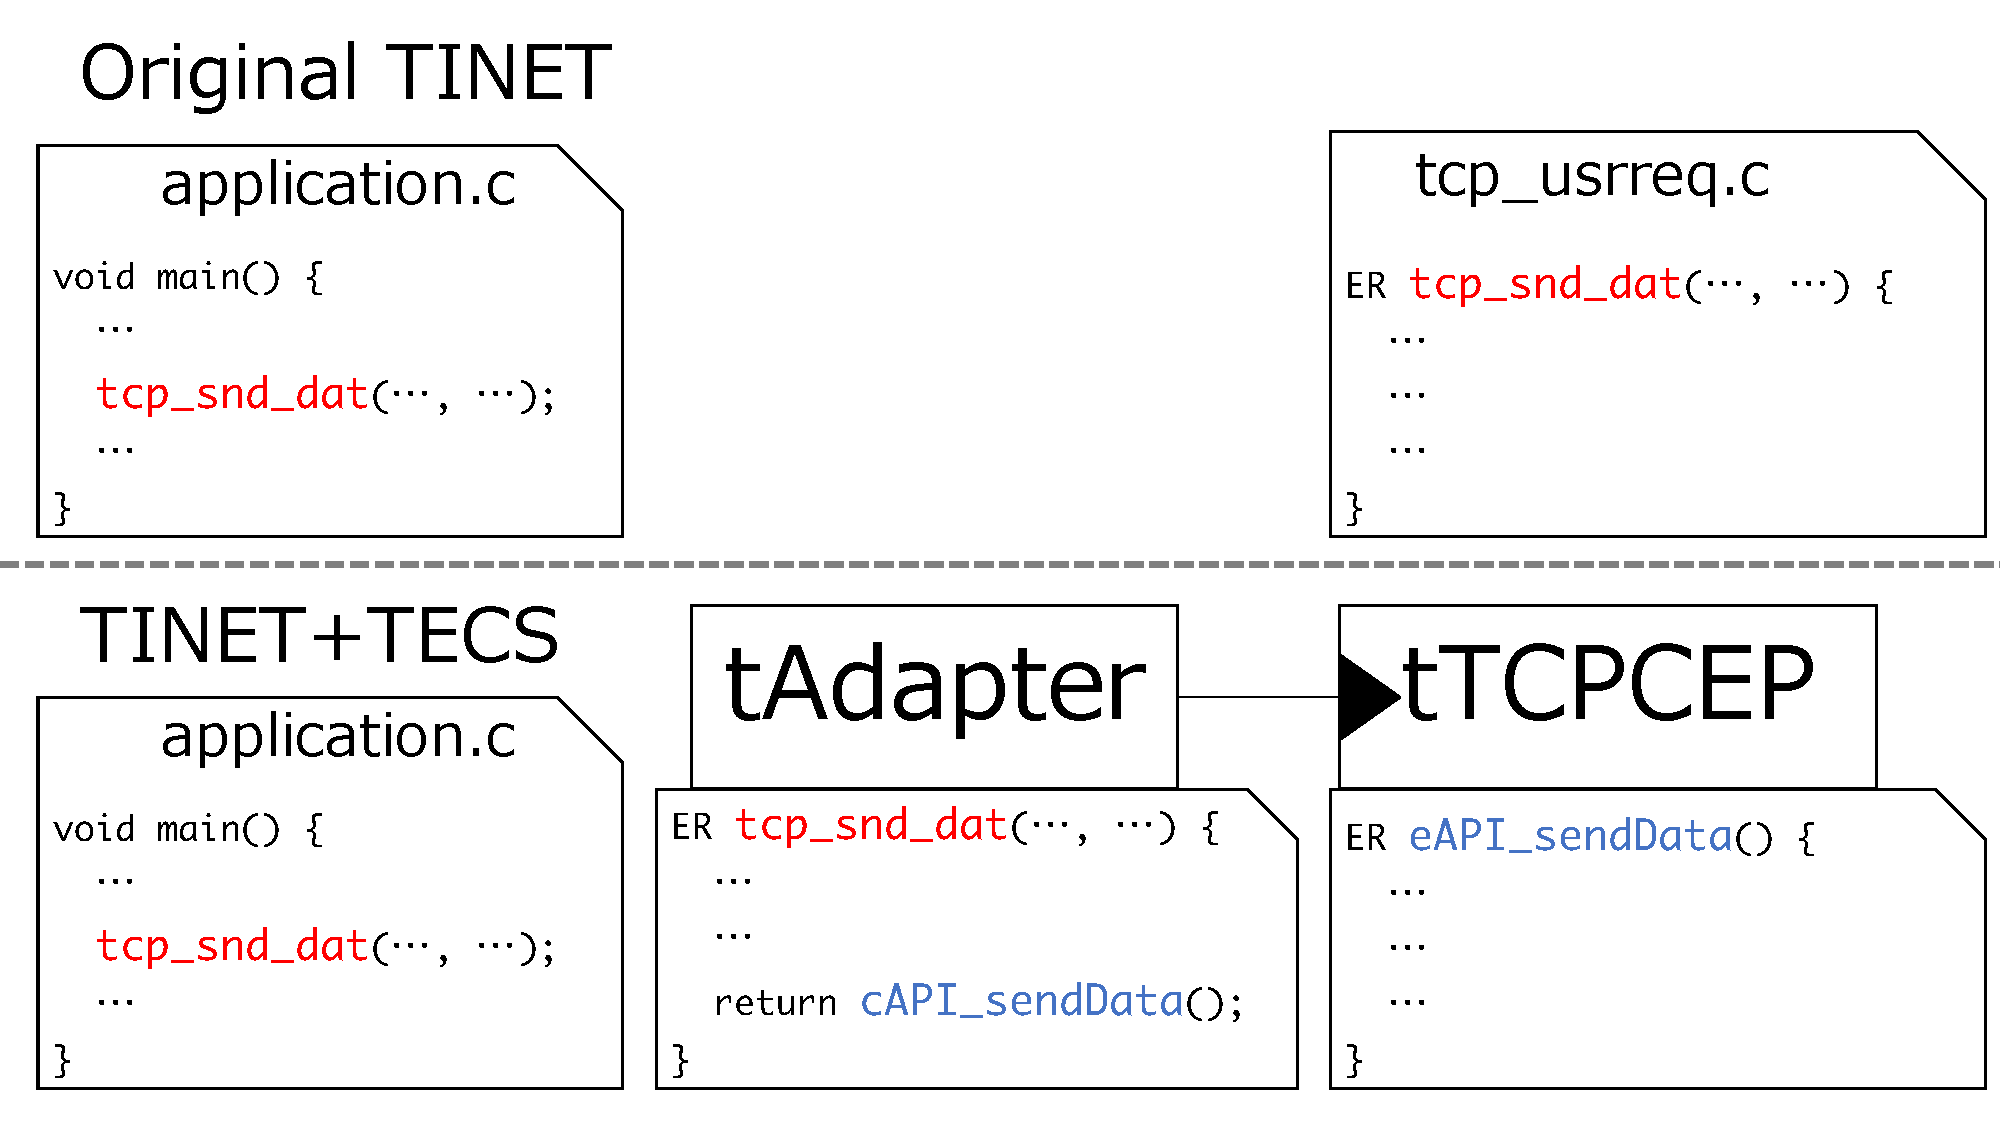
\includegraphics[width=6.5cm,clip]{figure/TECS_Adapter.pdf}
    \caption{TECS Adapter}
    \label{fig:TECS_Adapter}
\end{figure}




\section{Evaluation and Demonstration}
\label{sec:Evaluation and Demonstration}

\begin{table}[t]
    \centering
    \caption{Evaluation Board Environment}
    \begin{tabular}{l|l}
        \hline\hline
        Board           &   GR-PEACH                \\
        CPU             &   Cortex-A9 RZ/A1H 400MHz \\
        Flash ROM       &   8 MB                    \\
        RAM             &   10 MB                   \\
        LAN Controller  &   LAN8710A                \\
        \hline
    \end{tabular}
    \label{tab:Evaluation_Board_Environment}
\end{table}


\section{Related Work}
\label{sec:Related Work}

\section{Conclusion}
\label{sec:Conclusion}

% conference papers do not normally have an appendix


% use section* for acknowledgment
\section*{Acknowledgment}

% trigger a \newpage just before the given reference
% number - used to balance the columns on the last page
% adjust value as needed - may need to be readjusted if
% the document is modified later
%\IEEEtriggeratref{8}
% The "triggered" command can be changed if desired:
%\IEEEtriggercmd{\enlargethispage{-5in}}

% references section
\bibliographystyle{IEEEtranBST2/IEEEtran}
\bibliography{ref}

% that's all folks
\end{document}


